\documentclass[a4paper,12pt]{jarticle}

% レイアウト
\setlength{\hoffset}{0cm}
\setlength{\oddsidemargin}{-3mm}
\setlength{\evensidemargin}{-3cm}
\setlength{\marginparsep}{0cm}
\setlength{\marginparwidth}{0cm}
\setlength{\textheight}{24.7cm}
\setlength{\textwidth}{17cm}
\setlength{\topmargin}{-45pt}


\renewcommand{\baselinestretch}{1.6}
\renewcommand{\floatpagefraction}{1}
\renewcommand{\topfraction}{1}
\renewcommand{\bottomfraction}{1}
\renewcommand{\textfraction}{0}
\renewcommand\thefootnote{\arabic{footnote})}

% パッケージ
\usepackage[dvipdfmx]{graphicx}
\usepackage{amsmath,amssymb,epsfig}
\usepackage{eucal}
\usepackage{bm}
\usepackage{ascmac}
\usepackage{pifont}
\usepackage{multirow}
\usepackage{enumerate}
\usepackage{cases}
\usepackage{type1cm}
\usepackage{cancel}
\usepackage{url}
\usepackage{cite}
%\usepackage{color}
\usepackage[dvipdfmx]{color}
\usepackage{caption}
\usepackage[caption=false]{subfig}
\captionsetup[figure]{labelsep=space}

% 擬似コード作成用
\usepackage[ruled,vlined]{algorithm2e}
\usepackage{setspace}
\input{../sty/jdummy.def}

% カウンタの設定
\setcounter{section}{0}
\setcounter{subsection}{0}
\setcounter{subsubsection}{0}
\setcounter{equation}{0}

% キャプションの図をFigに変更
\renewcommand{\figurename}{Fig.}
\renewcommand{\tablename}{Tab.}

% 式番号を式(章番号.番号)に
\makeatletter
\renewcommand{\theequation}{\arabic{section}.\arabic{equation}}
\@addtoreset{equation}{section}
\makeatother

% 表紙
\title{\Large{電機システム制御特論\\ レポート課題3}
% {\large No title}
}
\author{\vspace{70mm}\\
九州工業大学\ \hspace{0mm} 工学府\\
機械知能工学専攻\ \hspace{0mm} 知能制御工学コース\\
\\
所属:\ 西田研究室\\
学籍番号:\ 17344219\\
提出者氏名:\ 二宮 \hspace{0mm} 悠二\\\vspace{5mm}\\}
\date{平成29年\ 5月\ 23日}

% ドキュメントの開始
\begin{document}
% 表紙
\titlepage
\maketitle
\thispagestyle{empty}
\newpage

% 目次
\thispagestyle{empty}
\tableofcontents
\newpage

% 課題内容
\section{課題内容}
%
次のシステムについて考える.
%
\begin{equation*}
 \begin{array}{c}
  \dot{x} = ax + bu + v \\
  y = x + w \\
 \end{array}
\end{equation*}
%
ただし,$ a = -0.02 , ~ b = 1.351 \times 10^{-3} $である.また,$ v $と$ w $は共に白色ガウス雑音であり,$ E \left\{v^2 \right\} = E \left\{w^2 \right\} = 0.7 $である.このとき,システム対するにカルマンフィルタを設計し,コンピュータシミュレーションによりその動作を示せ.


\section{カルマンフィルタ}
%
実用の際,様々な雑音が存在する/システムのパフォーマンスに影響を及ぼすような.
同一次元オブザーバはそれ自身が観測ノイズに対していくつかのフィルタ機能を持つものの,それはしばしば観測ノイズにふくまれた雑音成分を取り除くには不十分である.;確率システムに含まれるオブザーバゲインは与えられたノイズに対して最適化される可能性がある.
カルマンフィルタは,カルマン・ビュッスィー・フィルタとも呼ばれ,ホワイトガウシアンプロセスノイズのあるシステムの状態信号の最適な推定を行うことができる.



%
カルマンフィルタとは
白色ガウス雑音のあるシステムの状態信号の最適な推定値を与える.


ここで,次のような1入力1出力のシステムを考える.
%
\begin{eqnarray}
 \dot{x} & = & Ax + bu + v \\
 y & = &  cx + w
\end{eqnarray}
%
ただし,$ (A ,~ c) $は可観測である.$ v $はシステムノイズ,$ w $は観測ノイズである.
両ノイズは期待値に関係のある統計値として知られているホワイトガウシアンであるとみなされる.
すなわち,
%
\begin{equation*}
 \begin{array}{c}
  E\left\{v(t)\right\} = 0, ~~~ E\left\{w(t)\right\} = 0 \\
  E\left\{v(t) v(t)^T\right\} = Q \delta(t-\tau), ~~~ E\left\{w(t) w(t)^T\right\} = r \delta(t-\tau) \\
  E\left\{v(t)w(\tau)\right\} = 0 \\
 \end{array}
\end{equation*}
%
である.ただし,$ Q , ~~ r $は非負定値対称行列,$ \delta $はクロネッカーのデルタである.


定常カルマンフィルタは同一次元オブザーバと同様の構造で考えることができ,次のように表される.
%
\begin{eqnarray}
 \tilde{\dot{x}} & = &  A \tilde{x} + bu + l ( y - \tilde{y} ) \\
 \tilde{y} & = & \tilde{x}
\end{eqnarray}
%
カルマンゲインと呼ばれるフィードバックゲインは次の式で与えられる.
%
\begin{equation}
 l = \dfrac{1}{r} P c^T
\end{equation}
%
ここで,行列$ P $は推定誤差共分散と呼ばれ,次式のリッカチ方程式にて与えられる.
%
\begin{equation}
 AP + PA^T - \dfrac{1}{r}Pc^TcP = - Q
\label{riccati}
\end{equation}
%
このフィードバックゲインはシステム雑音と観測雑音から決定されるパラメータ$ Q $と$ r $の設計により最適化される.







\begin{figure}[b]
 \begin{center}
  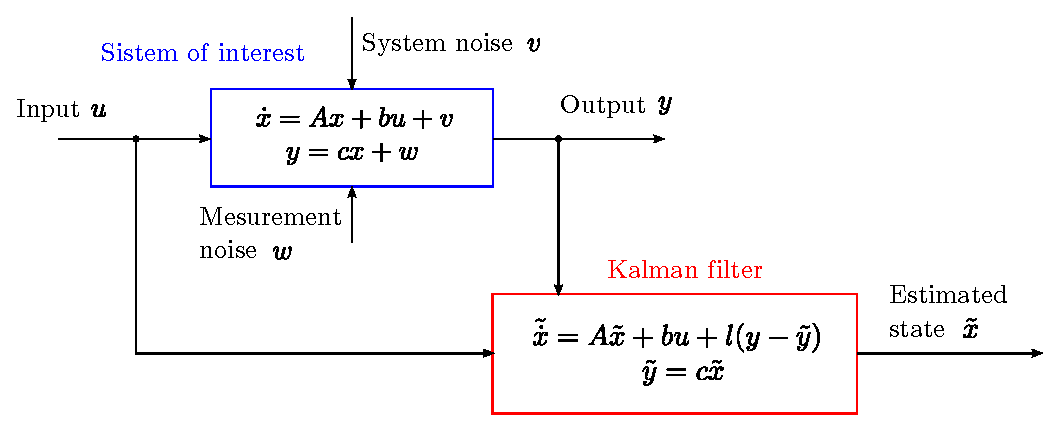
\includegraphics[scale=0.8]{../figure/eps/kalman.eps}
  \caption{カルマンフィルタを組み込んだ制御系}
  \label{kalman}
 \end{center}
\end{figure}
%

\subsection{ホワイトガウシアンノイズ}
%
白色ガウシアン雑音について説明する.

時系列$ y(k) $の分散が,

まず,白色雑音とは,
平均値がゼロで,$ w(t) $と$ w(\tau) $ $ (t \neq \tau ) $が無相関であることを言う.
特に白色ノイズ線形要素を通過したときの出力が正規分布,あるいはガウス分布に従うとき,入力である白色雑音は白色ガウス雑音と呼ばれる.


\subsection{離散時間カルマンフィルタ}
\subsection{離散時間定常カルマンフィルタ}
\subsection{連続時間カルマンフィルタ}
\subsection{連続時間定常カルマンフィルタ}

\section{シミュレーション}


\subsection{カルマンフィルタの設計}
%
本課題で与えられたパラメータを用いてカルマンフィルタを設計する.(\ref{riccati})式に数値を代入すると次のようになる.
%
\begin{equation}
 ap + pa - \dfrac{1}{r}p^2 = -q
\end{equation}
%
ここで,$ q $と$ r $はシステムノイズであり,共に 0.7 であるから,
%
\begin{equation}
 -0.04p - \dfrac{1}{0.7}p^2 = -0.7
\end{equation}
%
解の公式を用いてこの式を解くと,$ p > 0 $より
%
\begin{eqnarray}
 p & = & 0.68613 \cdots \nonumber \\
   & \simeq & 0.6861
\end{eqnarray}
%
を得る.以上から,カルマンゲイン$ l $は
%
\begin{eqnarray}
 l & = & \dfrac{1}{0.7} \times 0.6861 \\
   & = & 0.9801 \cdots\\
   & \simeq & 0.980
\end{eqnarray}
%
したがって,カルマンフィルタは次の式で与えられる.
%
\begin{equation}
 \begin{array}{rcl}
  \tilde{\dot{x}} & = &  -0.02 \tilde{x} + 1.351 \times 10^{-3} u + 0.980 ( y - \tilde{y} ) \\
  \tilde{y} & = & \tilde{x}
 \end{array}
\end{equation}
%



\subsection{検証}
%
前節で得たモデルを用いて MATLAB 上でシミュレーションを行い,その結果を出力した.その様子を{\bf Fig.}\ref{}に示す.


\section{考察・まとめ}
%
{\bf Fig.}\ref{}より,カルマンフィルタを用いることで観測ノイズを除去し,真値に近い値を推定できていることが分かる.




% % 図の挿入

% \begin{figure}[b]
%  \begin{center}
%   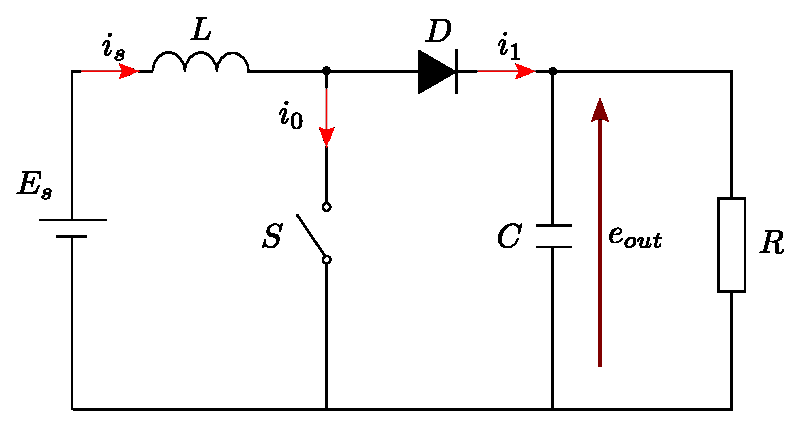
\includegraphics[scale=0.9]{../figure/circuit.eps}
%   \caption{Uncontrolled converter}
%   \label{circuit}
%  \end{center}
% \end{figure}


% % 表の挿入

% \begin{table}[htb]
%   \begin{center}
%     \caption{各素子のパラメータ}
%     \begin{tabular}{c|c|c} \hline
%       定数名[単位] & 記号 & 値 \\ \hline \hline
%       周波数[Hz] & $f_U,f_V,f_W$ & 120 \\ \hline
%                      & $\phi_U$ & $\frac{2\pi}{3}$ \\
%       初期位相角[rad] & $\phi_V$ & $\frac{4\pi}{3}$ \\
%                      & $\phi_W$ & $2\pi$ \\ \hline
%       抵抗[$\Omega$] & $R$ & 10 \\ \hline
%     \end{tabular}
%     \label{param}
%   \end{center}
% \end{table}


% % 図の挿入

% \begin{figure}[tb]
%  \centering
%  \vspace{0.5cm}
%  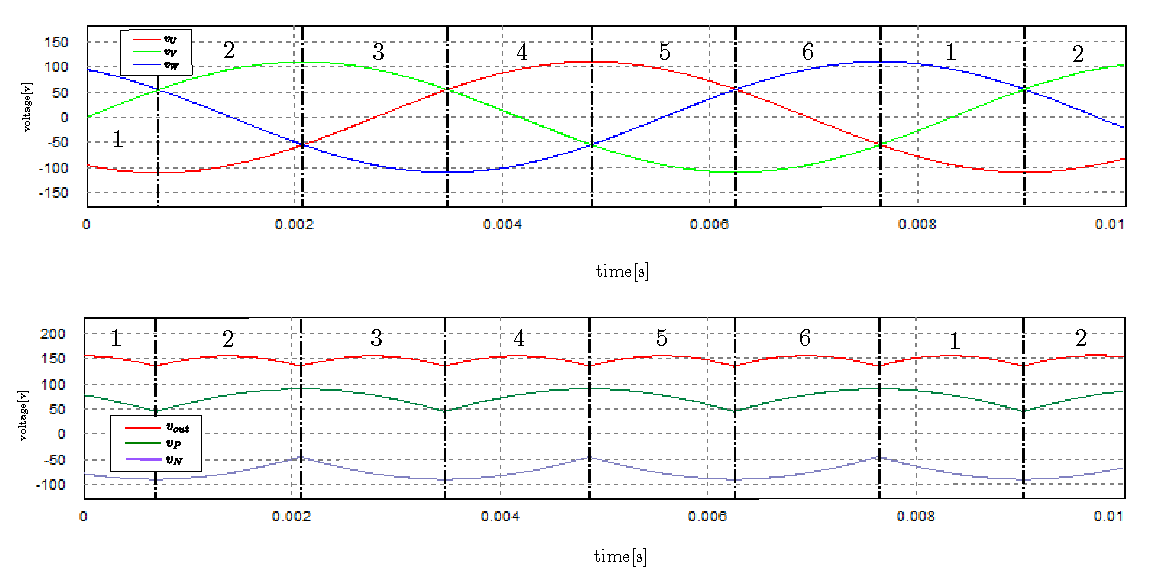
\includegraphics[scale=0.85]{../figure/waves.eps}\\
%  \hspace{0.0cm}
%  % 入力と出力\\
%  % \\
%  % \vspace{1.2cm}
%  % 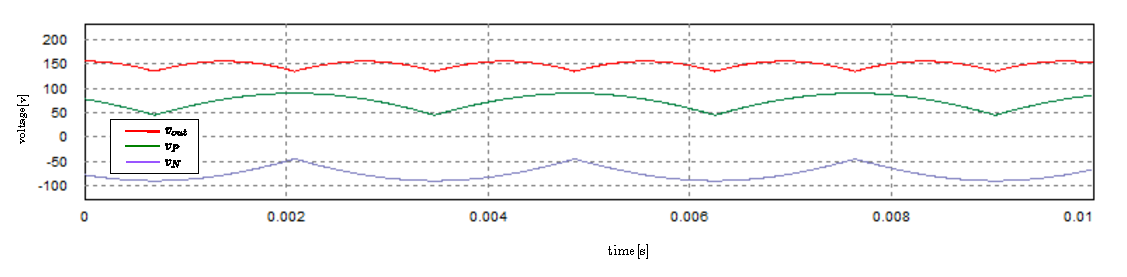
\includegraphics[scale=0.825]{../figure/output.eps}\\
%  % (b) 出力の電位\\
%  % \\
%  \caption{シミュレーションにより得られた各電源電圧(上)と出力電位(下)の波形}
%  \label{wave}
% \end{figure}

% \newpage

% % 図を並べて挿入

% \begin{figure}[tb]
%  \centering
%  \subfloat[区間1における回路動作]{\includegraphics[scale=0.5]{../figure/kukan_1.eps}}
%  \hspace{1.5cm}
%  \subfloat[区間2における回路動作]{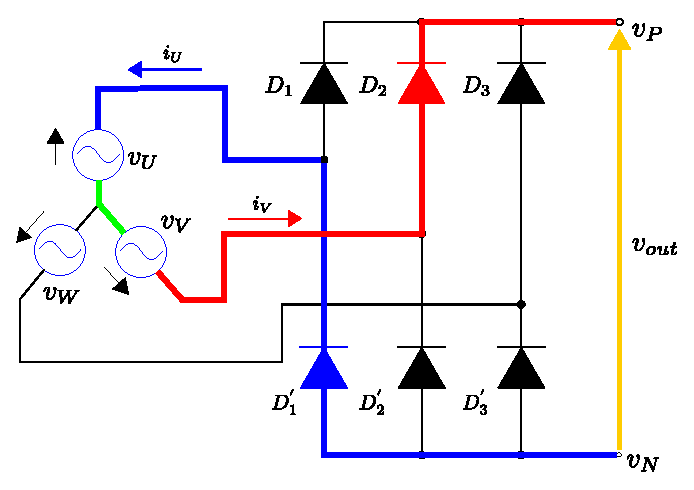
\includegraphics[scale=0.5]{../figure/kukan_2.eps}}
% \\
%  \vspace{0.5cm}
%  \subfloat[区間3における回路動作]{\includegraphics[scale=0.5]{../figure/kukan_3.eps}}
%  \hspace{1.5cm}
%  \subfloat[区間4における回路動作]{\includegraphics[scale=0.5]{../figure/kukan_4.eps}}
% \\
%  \vspace{0.5cm}
%  \subfloat[区間5における回路動作]{\includegraphics[scale=0.5]{../figure/kukan_5.eps}}
%  \hspace{1.5cm}
%  \subfloat[区間6における回路動作]{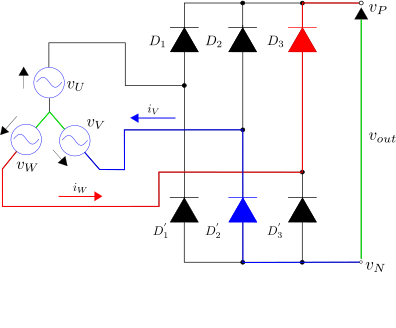
\includegraphics[scale=0.5]{../figure/kukan_6.eps}}
% \\
%  \caption{各区間での回路動作の様子}
%  \label{circuit_kaku}
% \end{figure}

% % 文中へのラベリング
% {\bf Fig. }\ref{circuit_kaku}に示す〜

% 参考文献
\begin{thebibliography}{99}
\addcontentsline{toc}{section}{参考文献}
\bibitem{1} T.Sakamoto,”Lecture Note of Advanced Electrical Drive Control System”,pp.44-46,2017.
\bibitem{2} 足立 修一,丸田 一郎,”カルマンフィルタの基礎”,東京電機大学出版局,pp.◯◯,2013.
\end{thebibliography}

\end{document}
